%%%%%%%%%%%%%%%%%%%%%%%%%%%%%%%%%%%%%%%%%%%%%%%%%%%%%%%%%%%%%%%%%%%%%%%%
%    INSTITUTE OF PHYSICS PUBLISHING                                   %
%                                                                      %
%   `Preparing an article for publication in an Institute of Physics   %
%    Publishing journal using LaTeX'                                   %
%                                                                      %
%    LaTeX source code `ioplau2e.tex' used to generate `author         %
%    guidelines', the documentation explaining and demonstrating use   %
%    of the Institute of Physics Publishing LaTeX preprint files       %
%    `iopart.cls, iopart12.clo and iopart10.clo'.                      %
%                                                                      %
%    `ioplau2e.tex' itself uses LaTeX with `iopart.cls'                %
%                                                                      %
%%%%%%%%%%%%%%%%%%%%%%%%%%%%%%%%%%
%
%
% First we have a character check
%
% ! exclamation mark    " double quote  
% # hash                ` opening quote (grave)
% & ampersand           ' closing quote (acute)
% $ dollar              % percent       
% ( open parenthesis    ) close paren.  
% - hyphen              = equals sign
% | vertical bar        ~ tilde         
% @ at sign             _ underscore
% { open curly brace    } close curly   
% [ open square         ] close square bracket
% + plus sign           ; semi-colon    
% * asterisk            : colon
% < open angle bracket  > close angle   
% , comma               . full stop
% ? question mark       / forward slash 
% \ backslash           ^ circumflex
%
% ABCDEFGHIJKLMNOPQRSTUVWXYZ 
% abcdefghijklmnopqrstuvwxyz 
% 1234567890
%
%%%%%%%%%%%%%%%%%%%%%%%%%%%%%%%%%%%%%%%%%%%%%%%%%%%%%%%%%%%%%%%%%%%
%
\documentclass[12pt]{iopart}
%\newcommand{\gguide}{{\it Preparing graphics for IOP journals}}
%Uncomment next line if AMS fonts required
%\usepackage{iopams}  

%\usepackage{subcaption}
%\captionsetup{compatibility=false}
\usepackage{subfig}
\usepackage[pdftex]{graphicx}
\usepackage{epstopdf}
\graphicspath{{./images/}{./images/other_formats/}}
\DeclareGraphicsExtensions{.pdf,.png,.eps,.jpg}

%Place footnotes at the bottom of the page
\usepackage[bottom]{footmisc}

\begin{document}

\title[]{A Modular and Cost-Effective Superconducting Generator Design for Offshore Wind Turbines}
\author{Ozan Keysan, Markus Mueller}

\address{Institute for Energy Systems,
University of Edinburgh, 
EH93JL, UK}
\ead{o.keysan@ed.ac.uk}
%\footnote{Supported by MARINA}

\begin{abstract}

Superconducting generators have the potential to reduce the tower head mass for large(\~ 10 MW) offshore wind turbines. However, a HTS generator should be as reliable as conventional generators for a successful entry to the market. Most of the proposed designs use the superconducting synchronous generator concept, which has a higher cost than conventional generators and suffer from reliability issues. In this paper, a novel claw-pole type superconducting machine is presented. The design has a stationary superconducting field winding, which simplifies the design and increases reliability. The machine can be operated in independent modules, thus even one of the sections fails the rest can operate at until next maintenance. Another advantage of the design is very low superconducting wire requirement; a 10 MW 10 rpm design is presented which uses 13 km of MgB2 wire at 30 K. The outer
diameter of the machine is 6.63 m and weighs 184 tonnes including the structural mass. The design thought to be a good candidate to enter the renewable energy market with its low cost and robust structure.

\end{abstract}

%Uncomment for PACS numbers title message
%\pacs{00.00, 20.00, 42.10}
% Keywords required only for MST, PB, PMB, PM, JOA, JOB? 
%\vspace{2pc}
%\noindent{\it Keywords}: Article preparation, IOP journals
% Uncomment for Submitted to journal title message
%\submitto{\JPA}
% Comment out if separate title page not required
\maketitle

\section{Introduction}

Average size of offshore wind turbines was 2~MW a decade ago, but now increased to 5~MW \cite{bvg}. The installation and maintenance cost of large offshore wind turbines are cheaper per MW compared to smaller wind turbines, and it takes less time to build a wind farm with larger turbines, which all help to reduce the cost of energy \cite{Bang2008}. It is aimed to build 10 MW, and even 20 MW, wind turbines \cite{upwind}, however, the tower head mass of larger wind turbines, which is estimated as 760 t for a 10 MW turbine, becomes a critical issue \cite{upwind}.

Direct-drive superconducting machines are proposed to minimize the tower head-mass and increase the energy yield \cite{Lesser2009, Lewis2007, Kalsi2004a}. It is stated in \cite{Lewis2007} that a 6 MW HTS direct drive generator may have 50 \% of the mass of a direct drive permanent-magnet generator and the lower mass of generator may enable transport and installation of the turbine in one piece.
In order to compare mass to torque ratio of HTS machines with other type of generators, data from direct-drive systems have been collected and the results are presented in a bubble chart in Figure \ref{generators_mass_comparison} and tabulated in Table \ref{generators_list}. Although, some designs are just conceptual designs and some are commercial products, the graph provides a good understanding of torque density capability of HTS machines.  The orange line represents ratio of generator mass to torque for permanent-magnet machines which is estimated as 25 kg/kNm by Bang \textit{et al.} in \cite{Bang2008}. The blue line represents the linear trend line estimated using the HTS machines in the graph. From the graph, it is clear that HTS machines are lighter than permanent-magnet generators for applications with torque requirements larger than 3000 kNm. The equation of the trend line can be represented as:

 \begin{equation}
     Mass(t)=0.011\times Torque(kNm)+45
     \label{mass_torque_eq}
 \end{equation}

\begin{figure}[]
\centering
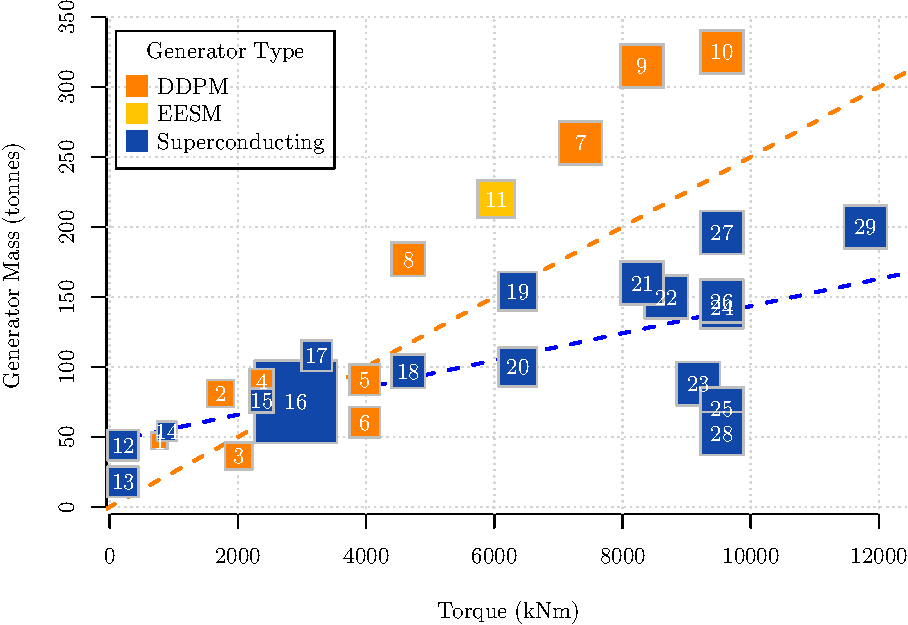
\includegraphics[]{generator_mass_compare}
\caption{Mass of different large direct-drive machines as a function of the torque, area of the square represents the power rating.
 DDPM: Direct drive permanent magnet generator, EESM: Electrically excited synchronous machine, Superconducting: High-temperature superconducting generator. Orange line represents generator mass to torque ratio ($m/T$) of 25 kg/kNm for permanent-magnet machines as given in \cite{Bang2008}. Blue line is the linear trend line for the superconducting machines.}
\label{generators_mass_comparison}
\end{figure}

\begin{table}[]
\begin{minipage}{\textwidth}
\caption{Torque density comparison conventional and superconducting generators.}
\label{generators_list}
\centering
\begin{tabular}{llcccrrl}
\hline
 & Manufacturer & Power & Speed & Mass & Torque & Mass/T & Type \\
&  & (MW) & (rpm) & (t) & (kNm) & (kg/kNm) & \\
\hline
1 & Harakosan \cite{Duan2009}& 1.5 & 18 & 47.2 & 796 & 59.3 & PMG \\
2 & The Switch \cite{Duan2009} & 3.8 & 21 & 81 & 1728 & 46.9 & PMG  \\
3 & NewGen \cite{Engstrom2004} & 4 & 19 & 36.4 & 2010 & 18.1 & PMG  \\
4 & NREL-AMSC \cite{Maples2010}& 3.1 & 12.5 & 90 & 2368 & 38.0 & PMG\footnote{The machine is not optimised for minimum mass.}  \\ 
5 & Bang et. al. \cite{Bang2009} & 5 & 12 & 90.8 & 3979 & 22.8 & TFPM  \\
6 &  & 5 & 12 & 60.5 & 3979 & 15.2 & TFPM\footnote{Ring-shaped TFPM.}  \\
7 & NTNU Reference \cite{Smith2012} & 10 & 13 & 260 & 7346 & 35.4 & PMG \\
8 & NREL-AMSC \cite{Maples2010} & 6 & 12.3 & 177 & 4658 & 38.0 &  PMG\footnote{The machine is not optimised for minimum mass.} \\
9 &  & 10 & 11.5 & 315 & 8304 & 37.9 & PMG\footnote{The diameter is limited to 4.3 m.}  \\
10 & Bang et. al. \cite{Bang2008} & 10 & 10 & 325 & 9549 & 34.0 & PMG \footnote{Estimated mass.}  \\
11 & Enercon-E126 & 7.5 & 12 & 220 & 6031 & 36.4 & EESM \\
12 & Lee et. al. \cite{Lee2008} & 5 & 230 & 44 & 208 & 212.0 & HTSG\footnote{Homopolar superconducting machine.}  \\
13 &  & 5 & 230 & 18 & 208 & 86.7 &  HTSG\footnote{Air-cored superconducting synchronous machine.} \\
14 &  Maki \cite{Maki2008} & 2 & 21.5 & 54 & 888 & 60.8 & HTSG  \\
15 & NREL-AMSC \cite{Maples2010} & 3.1 & 12.5 & 76 & 2368 & 32.1 & HTSG  \\
16 & AMSC \cite{Kalsi2006} & 36.5 & 120 & 75 & 2905 & 25.8 & HTSG \\
17 & Maki \cite{Maki2008} & 5 & 14.8 & 108 & 3226 & 33.5 & HTSG \\
18 & NREL-AMSC \cite{Maples2010}  & 6 & 12.3 & 97 & 4658 & 20.8 & HTSG  \\
19 & Maki \cite{Maki2008}  & 8 & 12 & 154 & 6366 & 24.2 & HTSG  \\
20 & Converteam \cite{Lewis2007} & 8 & 12 & 100 & 6366 & 15.7 & HTSG  \\
21 & NREL-AMSC \cite{Maples2010} & 10 & 11.5 & 160 & 8303 & 19.3 & HTSG  \\
22 & AMSC \cite{Snitchler2010} & 10 & 11 & 150 & 8681 & 17.3 & HTSG  \\
23 & Abrahamsen et. al. \cite{Abrahamsen2010}& 10 & 10.4 & 88 & 9182 & 9.6 & HTSG \footnote{The machine is found to be economically infeasible.} \\
24 & General Electric \cite{Fair2012} & 10 & 10 & 143 & 9549 & 15.0 & HTSG \footnote{The generator actually uses NbTi low temperature superconductor wire.} \\
25 & AML \cite{Masson2011} & 10 & 10 & 70 & 9549 & 7.3 & HTSG \footnote{Fully superconducting generator with MgB2 wires.} \\
26 & Sung et. al. \cite{Sung2013} & 10 & 10 & 147 & 9549 & 15.4 & HTSG \footnote{With YBCO wire.} \\
27 & & 10 & 10 & 196 & 9549 & 20.5 & HTSG \footnote{With Bi-2223 wire.} \\
\hline
\end{tabular}
\end{minipage}
\end{table}

Although, superconducting machines(including the cooling and other subsystems) become lighter than similar power-rated at larger  conventional generators (e.g. geared doubly-fed induction generators or direct-drive permanent magnet generators), low-mass is not the only desired property for offshore wind turbines. Firstly, offshore wind turbine generators operate in harsh conditions and are exposed significant vibration levels in the nacelle. Secondly, maintenance of offshore wind turbines are expensive and any failures result in long down periods adding lost generation income on top of the repair cost. Therefore, reliability and serviceability are very important for offshore wind turbines and in order to penetrate into the offshore renewable energy market, the superconducting generators should be as reliable and easy to maintain as the conventional generators. 
Compared to conventional generators superconducting generators have the disadvantage of having extra subsystems such as cryocooler, vacuum system etc. Therefore, any critical system should have redundancy to get fail-safe operation. It is desirable to have modularity in the power take-off system to make transportation, installation and maintenance easier.

The most common superconducting machine topology is the synchronous superconducting machine \cite{Gamble2011, Kalsi2004h}, which has a copper armature winding and a rotating DC-excited superconducting field winding, however, it may not be the most suitable topology for an offshore wind turbine application. The synchronous generator with a superconducting rotor has the following problems and challenges:

\begin{itemize}

  \item \textbf{Rotating Transfer Coupler:} In a rotating superconducting coil configuration, rotating transfer coupler introduces reliability issues and requires regular maintenance. Furthermore, it is the single point of failure for the whole generator system. Electric excitation system has the same problem.

  \item \textbf{Torque Transfer Structure:} Machines with rotating field superconducting winding require a torque transfer structure that is thermally insulating and structurally sound, which is difficult to design and expensive to manufacture.

  \item \textbf{Transient forces in the SC coil:} Second generation HTS tapes are prone to high stresses and bending. They are exposed to centrifugal and other transient forces in a rotating superconducting winding design.
  
  \item \textbf{Superconducting Wire Usage}: In a conventional synchronous superconducting machine, the magnetic flux has to cross the air-gap, vacuum and insulation layers. Thus, the equivalent magnetic gap is larger than the mechanical gap, which increases the superconducting coil requirement.
  
\end{itemize}

There are novel machine designs in literature aim to overcome some of these problems. AMSC plans to put the cold heads in the rotor for their 10 MW, 10 rpm generator design \cite{amsc_presentation}, but the design still requires cryocouplers. General Electric eliminated cryocouplers using a stationary superconducting coil and a rotating copper armature configuration \cite{Stautner2012}. In \cite{Chen2014}, a superconducting generator with stationary superconducting armature and field windings are shown, the machine is similar to a switched reluctance machine.

\section{Double Sided Claw Pole Concept}

In \cite{Keysan2011e, Keysan2012a} a radial flux claw pole machine is presented. The novelty of the design lays in having a single stationary superconducting field winding, which simplifies the cooling system. The rotor just consists of modular claw poles, which can be easily disassembled if required. In this paper, the radial flux claw pole machine is modified as shown in Figure~\ref{evolution_claw}.

\begin{figure}[]
  \centering
  \subfloat[Radial claw pole.]{\label{evolution_a}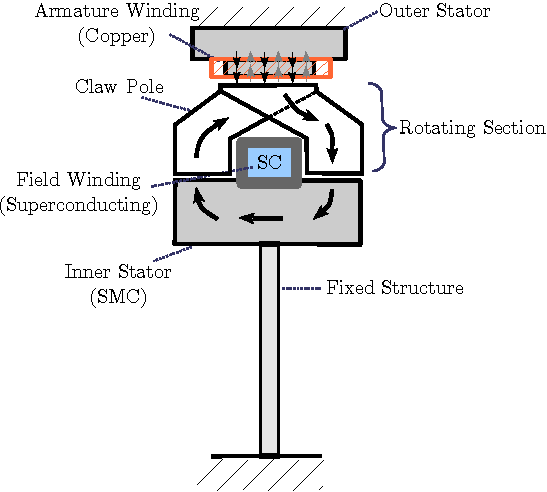
\includegraphics[scale=0.75]{radial_claw_pole}}
  \hspace{0.2in}
\subfloat[Axial claw pole.]{\label{evolution_b}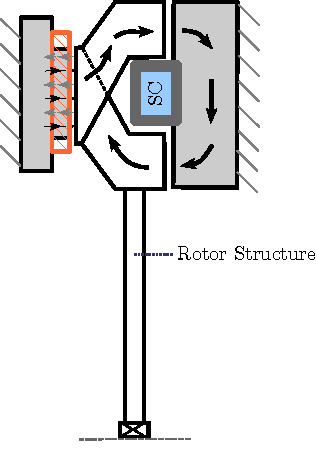
\includegraphics[scale=0.75]{axial_claw_pole}}
  
  \subfloat[Combined axial claw pole.]{\label{evolution_c}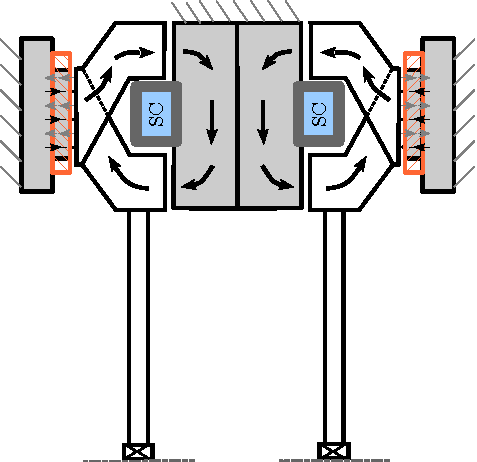
\includegraphics[scale=0.75]{double_axial_claw_pole}}
  \hspace{0.2in}
\subfloat[Double-sided claw pole.]{\label{evolution_d}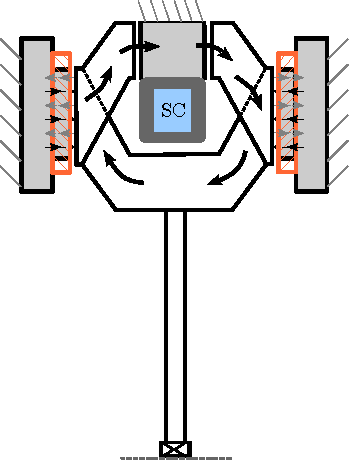
\includegraphics[scale=0.75]{double_claw_pole}}
    \caption{Evolution of the claw pole topology.} 
    \label{evolution_claw}
\end{figure}

The advantages of the double-sided claw pole topology compared to other superconducting machine designs can be listed as:

\begin{itemize}
  \item The machine has a stationary superconducting field winding, which means: no cryocoupler, no brushes or brushless exciters, no vibrational or rotational forces acting on the SC coil.
  \item The magnetic attraction forces on the rotor structure are symmetrical and cancel each other, which means reduced structural mass.
  \item The machine has two armature windings that can be operated independently. Thus, the modularity is increased.
  \item The machine uses significantly less superconducting coil due to iron-cored structure and loop-shaped field winding.
\end{itemize}

The machine analysed using 3D finite-element software and the flux density vectors in the machine are presented in Figure~\ref{double_claw_parts}. The flux density vectors shown in Figure~\ref{double_claw_B_vector_iso} verify the operation of the proposed topology, as the magnetic flux created by the superconducting coil links both armature cores through the claw poles as depicted in Figure~\ref{evolution_d}.

\begin{figure}[]
  \centering
  \subfloat[Section of the machine.]{\label{double_claw_parts_iso}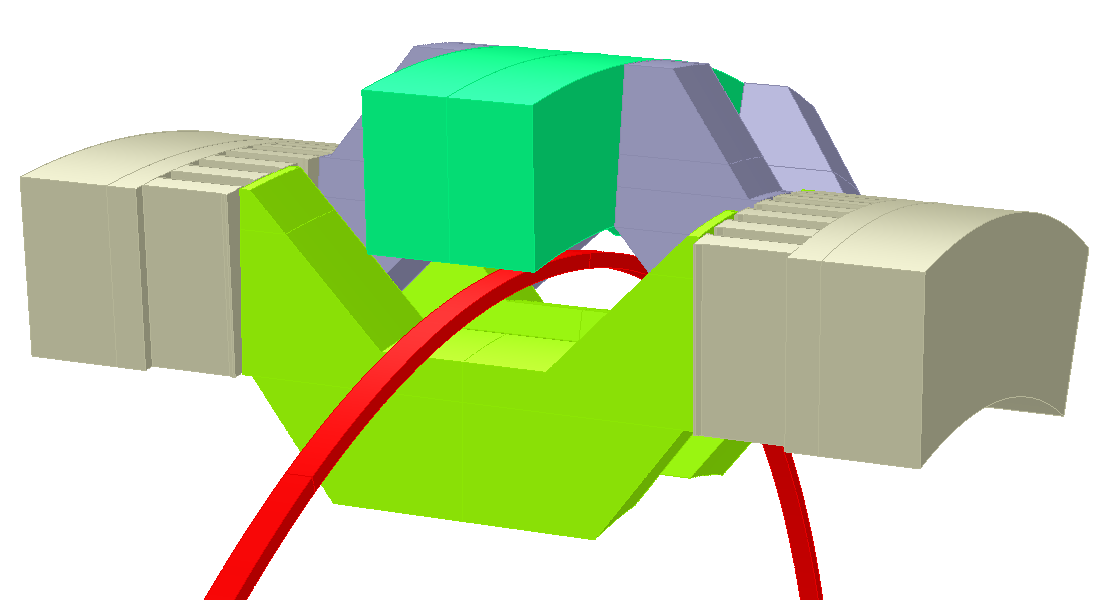
\includegraphics[scale=0.75]{double_claw_parts_iso}}
\hspace{0.5in}
\subfloat[Full machine.]{\label{double_claw_full}   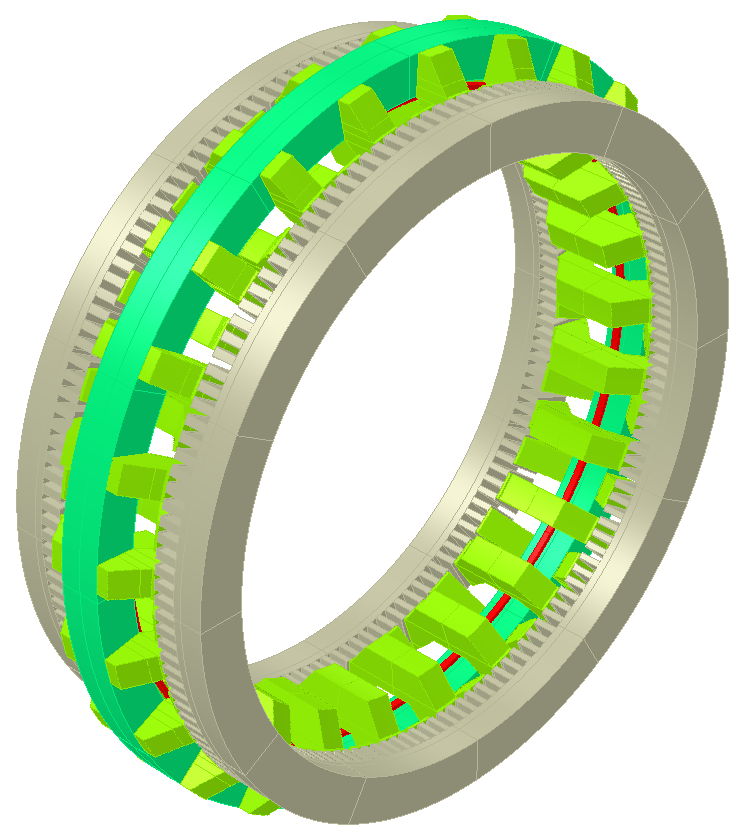
\includegraphics[scale=0.75]{double_claw_full}}

\subfloat[Flux density vectors.]{\label{double_claw_B_vector_iso}   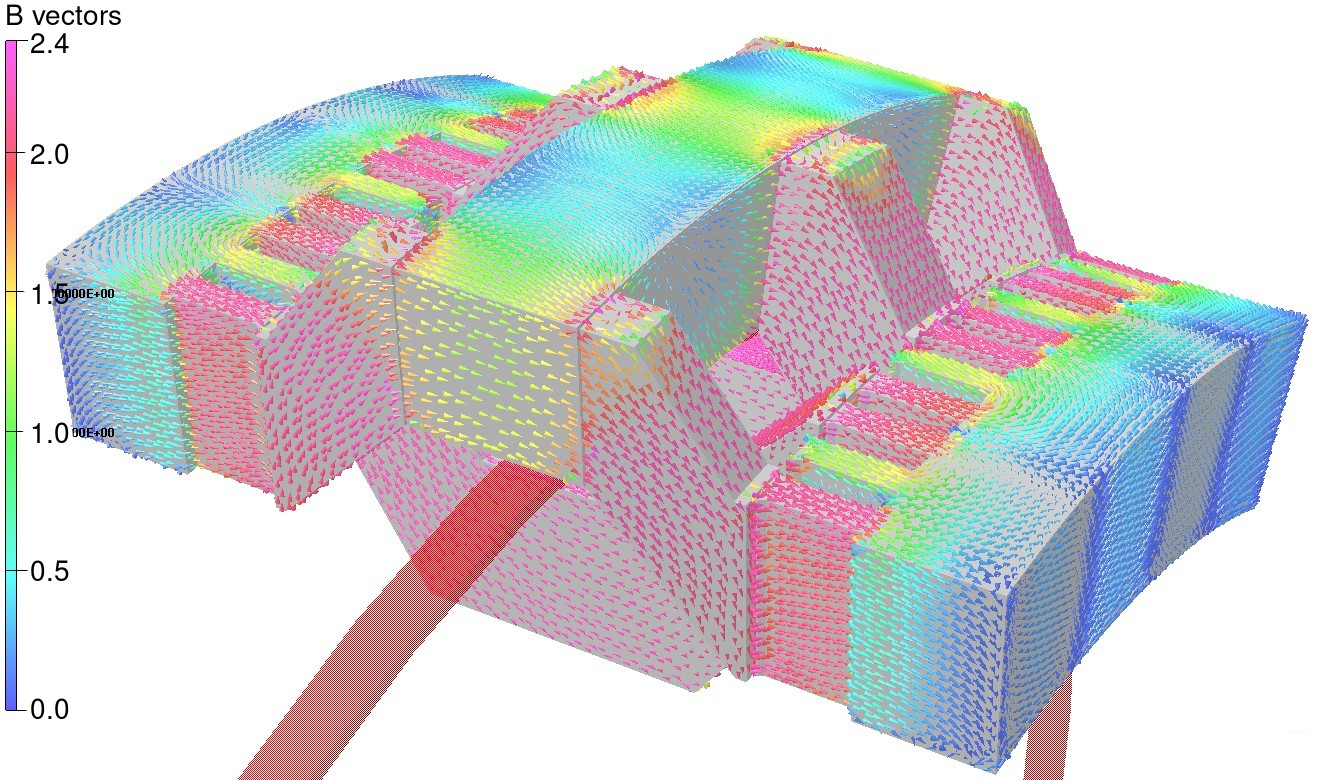
\includegraphics[scale=0.75]{double_claw_B_vector_iso}}

  \caption{The double-claw pole machine model and flux density vectors.} 
  \label{double_claw_parts}
\end{figure}

\subsection{Material Selection}

Power density of the machine is limited by magnetic saturation as it is iron-cored, which makes the material selection very critical.  Vacuumschmelze introduced a cobalt-iron alloy called VacoFlux50, which can be manufactured in laminations and has an impressive magnetic saturation limit with 2.35 T at 16 kA/m \cite{vacoflux}. VacoFlux50 has satisfactory mechanical properties with a Young's modulus of 210 kN/mm$^2$ and tensile stress of 350 N/mm$^2$ \cite{vacoflux}.  VacoFlux50 has a few variants, such as VacoDur with improved mechanical strength and VacoFlux17 with lower cost. This material is promising for superconducting machine designs with its high saturation limit and used in the calculations in this paper. 

\subsection{Sectioned Cryostat}

Although, the initial design has a single loop-shaped superconducting field winding, it is difficult to manufacture and install the field winding in one piece in multi-MW scale. In the original design, the cryostat is fixed to the inner surface of the field core as shown in Figure~\ref{single_cryostat}, however, it is also possible to mount another coil on the outer surface of the field core as in Figure~\ref{double_cryostat}. Then, the cryostat can be divided into smaller sections as shown in Figure~\ref{sectioned_cryostat}. This configuration has two main advantages. Firstly, it is easier to manufacture and install the sectioned cryostat compared to full span cryostat. Secondly, two independent cryostat introduces modularity to the system, thus even one of the cryostats fails  the machine can still operate at half-capacity until maintenance.
 
\begin{figure}[]
  \centering
  \subfloat[Single cryostat.]{\label{single_cryostat}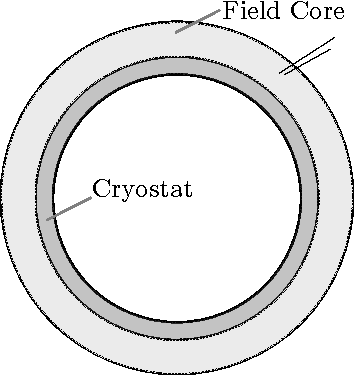
\includegraphics[scale=0.7]{single_cryostat}}  \hfill
  \subfloat[Double cryostat.]{\label{double_cryostat}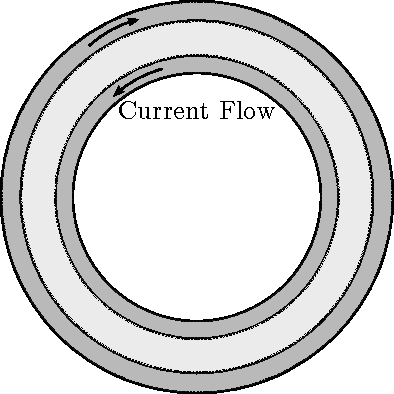
\includegraphics[scale=0.7]{double_cryostat}} \hfill 
  \subfloat[Sectioned cryostats.]{\label{sectioned_cryostat}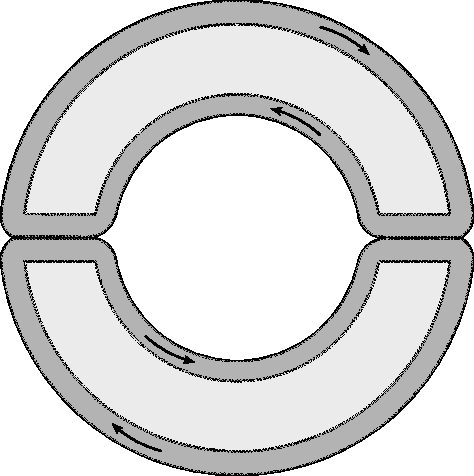
\includegraphics[scale=0.6]{sectioned_cryostat}}
    \caption{Sectioned cryostat design for the double-claw pole machine.} 
    \label{cryostat_variants}
\end{figure}

\section{Design of a 10 MW Superconducting Generator}
 
As presented in the introduction section and in Table~\ref{generators_list}, 10~MW, 10~rpm superconducting generator designs are quite common in the literature, therefore, a 10 MW double-sided claw pole machine is designed for a better comparison with other superconducting machine designs.

A parametrized FEA model of the proposed topology is developed, which estimates the air gap flux density and power output. The machine is optimized using the genetic algorithm optimization tool ``rgenoud'' \cite{Mebane2011}. 
The objective function is defined as the total active material mass, with pre-defined constraints in outer diameter, phase voltage and current density.
%More details can be found on optimization algorithm in \cite{github-repo}.


The main specifications of the optimum design is presented in Table \ref{10MW_spec} and the outline is shown in Figure \ref{10MW_drawing}. The machine has an outer diameter of 6.6 m and an axial length of 1.4 m, which is a similar size to a 5 MW direct-drive permanent magnet generator. The machine has an electrical frequency of 7.33 Hz. There are 11 coils in series and two parallel branches for each phase.

\begin{table}[]
  \centering
  \begin{tabular}{ll}
\hline
Power Rating & 10 MW \\
Rotational Speed & 10 rpm \\
Number of Poles & 88 \\
\hline
Outer Diameter & 6.63 m \\
Armature Diameter & 5.84 m \\
Rotor Radius & 3.20 m \\
Inner Radius & 2.29 m \\
Axial Length & 1.38 m \\
\hline
Number of Stator Slots & 66 \\
Number of Turns & 96 \\
Induced Coil Voltage & 173 V$_{rms}$\\
Phase Voltage Voltage & 3.3 kV$_{ll}$ \\
\hline
 \end{tabular}
  \caption{Main specifications of the optimized 10 MW, 10 rpm design.}
  \label{10MW_spec}
\end{table}

\begin{figure}[]
  \centering
    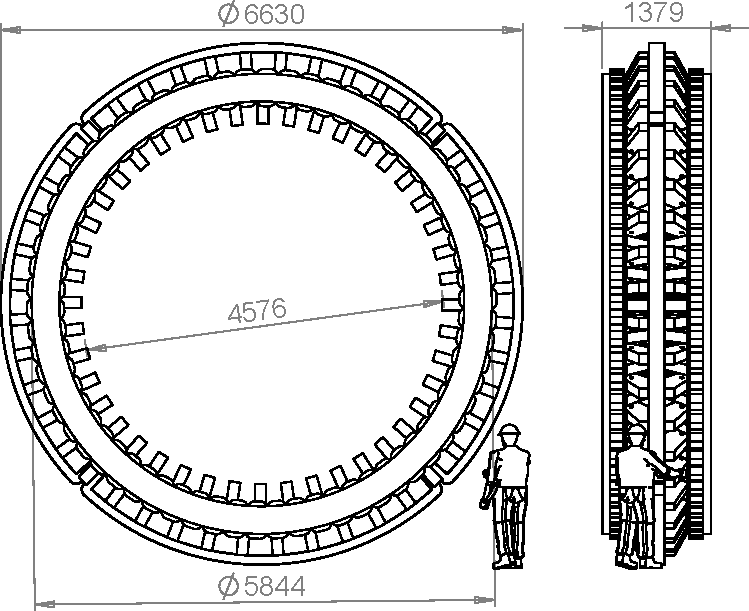
\includegraphics[]{10MW_outline_drawing}
  \caption{The outline dimensions of the 10 MW, 10 rpm generator design. Dimensions are in mm.}
  \label{10MW_drawing}
\end{figure}

Figure~\ref{10MW_tooth_Bz} shows the flux density distribution in the stator tooth when the large claw pole and small claw pole are aligned with the middle stator tooth. 

\begin{figure}[]
  \centering
  \subfloat[Middle tooth aligned with the large claw pole.]{\label{Bz_0_deg}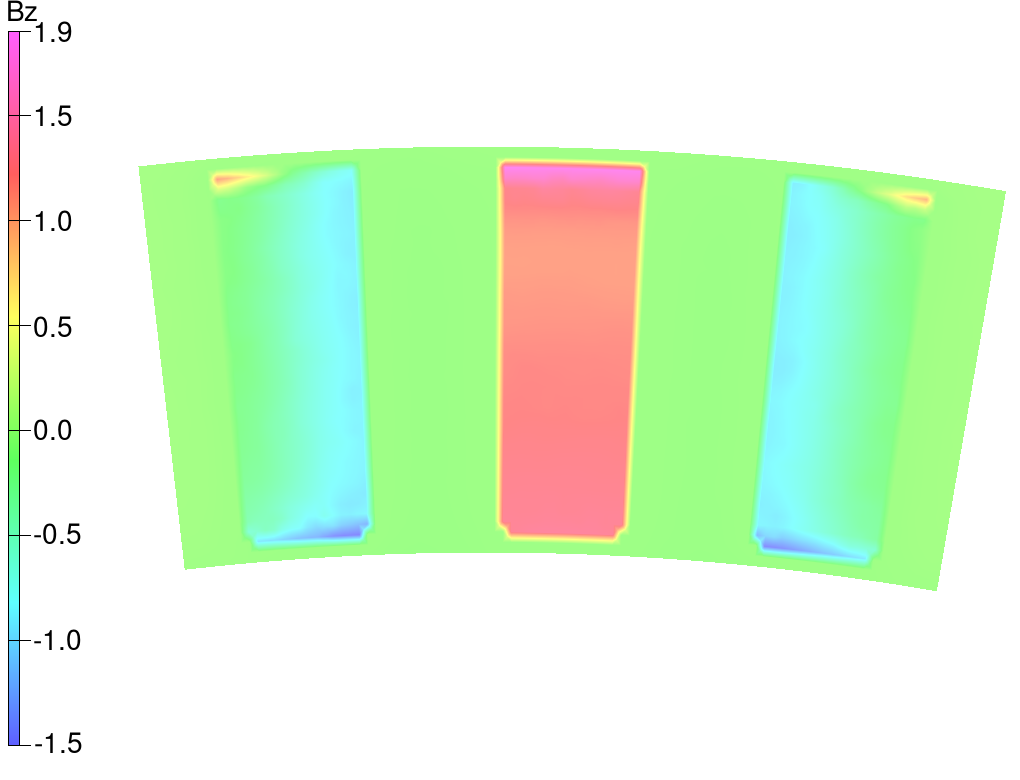
\includegraphics[]{Bz_0_deg}}
  \hfill
  \subfloat[Middle tooth aligned with the small claw pole.]{\label{Bz_90_deg}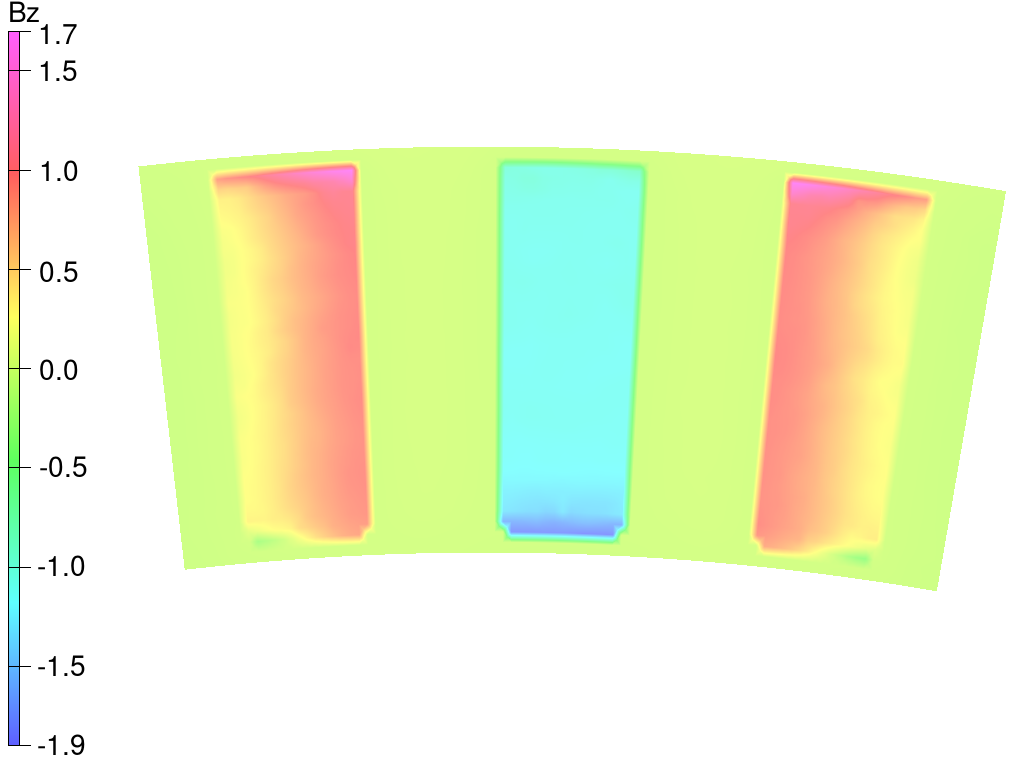
\includegraphics[]{Bz_90_deg}}
   \caption{Flux density distribution in Z direction (into the page) in the stator teeth at mean coil radius.} 
    \label{10MW_tooth_Bz}
\end{figure}

\subsection{Mass Estimation}


The excess structural mass in the large direct-drive generators is a serious issue. Although, the proposed machine has a smaller diameter than equivalent DDPM generators, which helps to reduce the structural mass, the high air-gap flux density increases the stress on the mechanical structure.

It is possible to install the proposed generator in two different configurations as shown in Figure~\ref{DD_claw_pole_structures}: axial armature winding or radial armature winding. In this paper, axial armature configuration is used for mass calculations, which are presented in Table~\ref{10MW_total_mass}. The total mass of the generator is estimated as 184 tonnes. The structural mass dominates the total mass by 68 \%.

\begin{figure}[]
  \centering
  \subfloat[Axial armature winding, inner rotor.]{\label{structure1}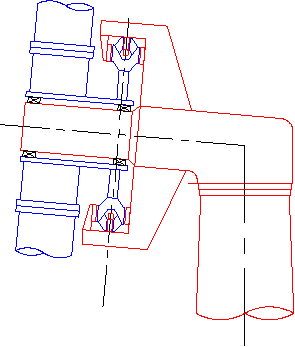
\includegraphics[]{structure_claw_radial_inner}}
  \hfill
  \subfloat[Radial armature winding.]{\label{structure2}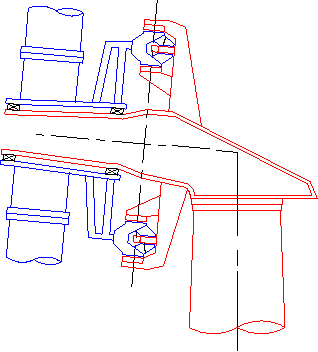
\includegraphics[]{structure_claw_axial}}
   \caption{Two possible configurations for the installation of double-claw pole machine to a wind turbine (Drawings modified from \cite{Bang2010}).} 
    \label{DD_claw_pole_structures}
\end{figure}


\begin{table}
  \centering
  \begin{tabular}{lr}
\hline
Small Claw Pole & 114 kg \\
Large Claw Pole & 314 kg \\
\hline
Rotor Structure & 42.8 t \\
Stator Structure & 83.5 t \\
\hline
Magnetic Core & 52.4 t\\
Copper & 2.3 t\\
Cooling - Cryostats & 3.2 t \\
\hline
Total Mass & 184.2 t \\
\hline
 \end{tabular}
  \caption{The structural and active material mass estimations for the 10 MW, 10 rpm machine.}
  \label{10MW_total_mass}
\end{table}


\subsection{Estimation of Losses}

Main losses in the machine are presented in Table~\ref{10MW_efficiency}. Phase resistances are calculated conductor dimensions and number of turns. Current density in the conductor is assumed as 5 A/mm$^2$. Copper armature winding dissipates 510 kW of heat loss, which is cooled down by 40 kW of air blowers. The core loss in the field core and stator core is calculated
as 7 kW by extrapolating the core loss values presented in VacoFLux datasheet for 7.3 Hz, which is the electrical frequency in the machine at 10 rpm. Eddy current losses in the armature winding is neglected due to the low electrical frequency. Power requirement for the cryocoolers will be estimated in the next section.

\begin{table}[]
  \centering
  \begin{tabular}{lr}
\hline
%Input Power & 10,571 kW \\
%Pin=9987+510+7+24+30
Copper Loss & 510 kW \\
Core Loss & 7 kW \\
Cryocoolers & 24 kW \\
Air Blowers (Armature) & 40 kW \\
%Output Power & 9,987 kW \\
\hline
Efficiency & 94.5 \% \\
%9987/10571
\hline
\end{tabular}
  \caption{Main losses and efficiency estimation for the 10 MW, 10 rpm design.}
  \label{10MW_efficiency}
\end{table}

It is important to accurately estimate the heat leakage in the cryostats, which can be divided into gas heat conduction through the vacuum, radiation heat from  warm walls of the cryostat, conduction through superconducting coil mechanical support, heat leakage through current leads and eddy current loss. These losses are estimated using the methodology presented in \cite{Abrahamsen2012, Simons2013}. 

%The operating temperature is assumed as 30 K.

The surface area of a single cryostat is 6.1 $m^2$, which gives the total cryostat wall area as 24.4 $m^2$. The cryostat used in the proposed generator is different to a superconducting rotor, where a cylindrical cryostat is used. Assuming a 5 m diameter, surface area of a cylindrical cryostat can be calculated as 55 $m^2$, which is twice the area of the proposed cryostat. Thus, the heat loss through cryostat wall is lower.

The heat loss can be calculated as shown in \cite{Ekin206}. The operating pressure is chosen as 10\textsuperscript{-3} Pa, which can be achieved using standard industrial equipments. The heat loss at this vacuum level is 3.9 W. Radiation loss is calculated as 17.5 W by using 10 mm of MLI insulation, which has 30 layers.

Suspension straps are required to mechanically support the superconducting coil. As there are no electromagnetic torque acting on the superconducting coil, the design of these suspension straps relatively straightforward compared to the torque tubes of other types of superconducting machines. The distance between suspension straps is assumed as 1 m, which gives 10 straps per cryostat. Assuming the straps are made of G10-CR fibreglass, the conduction heat loss can be calculated as 13.5 W per cryostat.

The length of current leads should be carefully assessed as it depends on two factors: resistive losses and heat conduction through ambient. For minimum losses, the resistive and conductive losses should be equal as presented in \cite{Kalsi2011a}. Assuming a current input of 90 A, the heat loss in a single current lead is found as 5.9 W (11.8 W per cryostat).

Total heat losses in the cryostats are tabulated in Table \ref{10MW_thermal_budget}. The heat loss at 65 K is also presented, which is estimated as 154.2 W. The total thermal budget of the machine  at 30 K is 157.2 W, slightly larger than the heat loss at 65 K. Adding 25\% safety margin, the machine can be cooled using 4~x~50~W cryocoolers. A suitable cooling system for such a requirement is selected as Cryomech's Gifford-McMahon AL230 cold-head coupled with CP950 compressor, which can supply 60 W of cooling power at 30 K \cite{Cryomech2007}. Total cooling system mass in the generator is calculated as 2,000 kg with an electrical power input of 24 kW.

To summarize, the proposed topology has the advantage of independent cryostats, which increases the modularity and overall availability of the system. The total cryostat wall area is smaller compared to the conventional cylindrical cryostats, which helps to reduce the gas conduction and radiation losses. However, the sectioned cryostat results in higher number of current leads and suspension straps which increases the conduction losses. In general, the heat loss is within the reasonable values. For example in \cite{Snitchler2011}, it is stated that six to ten CTI-1020 cryogenic coolers are used for AMSC's 10 MW superconducting generator, provides 280--450 W of cooling power.
In \cite{Stautner2012}, the total cooling requirement for the GE's 10 MW LTS superconducting generator is estimated as 131 W, and in \cite{Abrahamsen2012}, 500~W is defined as the upper limit of the cooling power for a 5~MW superconducting generator.

\begin{table}
  \centering
  \begin{tabular}{lrr}
& 30 K & 65 K \\
& MgB2--90 A & YBCO--120 A \\
\hline
Gas Conduction (at $10^{-3}$ Pa) & 3.9 W & 3.4 W\\
Suspension Straps & 54.0 W & 50.0 W\\
Radiation & 17.5 W & 17.4 W\\
Current leads & 47.2 W & 48.8 W \\
Cold-head sleeve & 15.6 W & 15.6 W\\
Eddy Current & 4.0 W & 4.0 W\\
Other & 15.0 W & 15.0 W\\
\hline
Total loss & 157.2 W & 154.2 W\\
\hline
 \end{tabular}
  \caption{Thermal budget for the 10 MW, 10 rpm design. }
  \label{10MW_thermal_budget}
\end{table}

\subsection{Superconducting Coil Requirements}

The magneto-motive-force of the superconducting coil is selected by the optimisation algorithm as 32.4 kAt, which saturates the claw poles up to 2.3 T. Total superconducting coil requirement in four cryostats (4~x~10.4~m) can be calculated as 1348 kAt.m as shown in Table~\ref{10MW_hts_spec}. In the calculations, data from AMSC's Amperium YBCO wire \cite{AMSC2012} and MgB2 wires manufactured by Columbus Superconductor \cite{Modica2006} have been used.

\begin{table}[]
  \centering
  \begin{tabular}{ll}
\hline
Mean turn length & 10.4 m \\
MMF of the SC & 32.4 kAt \\
Number of Cryostats & 4 \\
Total SC requirement & 1348 kAt.m \\
\hline
 \end{tabular}
  \caption{Superconducting winding specifications for the 10 MW, 10 rpm design.}
  \label{10MW_hts_spec}
\end{table}

\begin{table}[t]
  \centering
  \begin{tabular}{lccc}
& MgB2 & \multicolumn{2}{c}{YBCO} \\
\hline
Operating Temperature & 30 K & 30 K & 65 K \\
Current ($~0.8I_c$) & 90 A & 400 A & 100 A \\
Number of turns & 360 & 81 & 324 \\
Wire thickness & 0.67 mm & 0.22 mm & 0.22 mm \\
Wire width & 3.65 mm & 4.8 mm & 4.8 mm \\
Wire length(per cryostat) & 3744 m & 842 m & 3370 m \\
Wire length (total) & 15.0 km & 3.4 km & 13.5 km \\
\hline
 \end{tabular}
  \caption{Superconducting tape requirements for the 10 MW, 10 rpm design (MMF=32.4~kAt).}
  \label{10MW_hts_wire_spec}
\end{table}

Three cases are investigated for the superconducting coil: MgB2 at 30 K, YBCO at 30 K, YBCO at 65 K. In critical current calculations, magnetic flux penetrating into the superconducting coil is taken into account. In \cite{Keysan2012a} it is found that, magnitude of the perpendicular penetrating flux is less than 0.03 T and the magnitude of the parallel flux component in the SC coil is around 0.36 T. Critical current at each temperature is reduced in proportion using the material data-sheets for penetrating flux values.

The required superconducting wire lengths are presented in Table~\ref{10MW_hts_wire_spec}. In Table~\ref{SC_length_compare}, SC wire requirements of several 10 MW designs are compared. Table shows the SC wire requirement is substantially less than other superconducting designs. In particular, air-cored topologies require hundreds of kilometres of superconducting wire. The closest design is the AMSC \cite{Snitchler2011}, which requires 36 km of YBCO at 30 K. However, the proposed design just requires 3.4 km of YBCO in total at that temperature, which is less than one tenth of the AMSC's design.

\begin{table}[]
\caption{Comparison of superconducting wire requirements and total mass of 10~MW direct-drive superconducting generators.}
\label{SC_length_compare}
\centering
\begin{tabular}{lcr}
\hline
 & SC Wire Requirement & Total Mass \\
\hline
		& 15 km MgB2 (30 K) & \\
Proposed Design	& 3.4 km YBCO (30 K) & 184 t\\
 		& 13.5 km YBCO (65 K) & \\
\hline
\hline
Abrahamsen et. al. \cite{Abrahamsen2010} & 200--300 km YBCO &88 t\\
General Electric \cite{Fair2012} & 720 km NbTi & 143 t \\
AMSC/Snitchler et. al. \cite{Snitchler2011}  & 36 km YBCO (30K) & 150 t \\
Sung et. al. \cite{Sung2013} & 586 km YBCO & 147 t \\
Sung et. al. \cite{Sung2013}& 222 km Bi2223 & 196 t \\
Terao et. al. \cite{Terao2012} & 270 km HTS + 275 km MgB2 & - \\
Kim et. al. \cite{Song2012}& 919 km HTS & - \\
Quddes et. al. \cite{Quddes2011} & 1050--1400 km HTS & - \\
\hline
\end{tabular}
\end{table}

The low SC requirement is due to two main reasons. Firstly, the coil is loop shaped, which results in better utilization of the MMF per length of the coil. Secondly, as shown in Figure~\ref{magnetic_mechanical_gap}, the magnetic gap in the claw pole topology equals to the mechanical gap. However, in a typical superconducting machine the flux has to pass through many layers (vacuum, radiation shield, EM shield, etc.) through the cryostat, which results in a much larger magnetic gap and increased MMF requirement.

\begin{figure}[]
  \centering
  \subfloat[Synchronous machine with superconducting rotor.]{\label{standard_hts_machine_gap}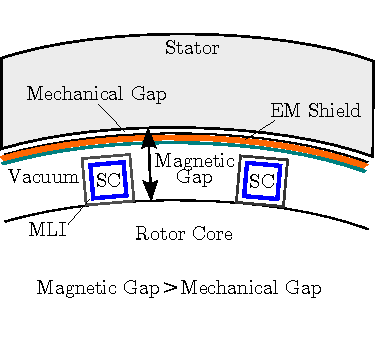
\includegraphics[scale=0.8]{standard_hts_machine_gap}}
  \hspace{0.5in}
  %\hfill
  \subfloat[Claw pole superconducting machine.
]{\label{claw_pole_gap}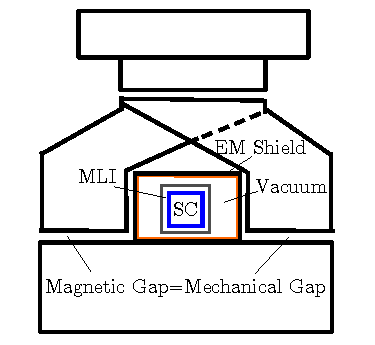
\includegraphics[scale=0.8]{claw_pole_gap}}
    \caption{Magnetic and mechanical gap comparison for the typical superconducting machine and the claw pole machine.} 
    \label{magnetic_mechanical_gap}
\end{figure}


\section{Conclusion}

This paper presents a novel superconducting machine design by introducing the stationary superconducting field winding concept. The concept simplifies the cryostat design by eliminating the transfer couplers and any rotating parts, which helps to increase the reliability. Furthermore, a sectioned cyryostat concept is also presented. This improves modularity and redundancy to the system, which is critical for offshore wind turbines where the O\&M is difficult and expensive.

Maybe the biggest advantage of the proposed topology is the minimal superconducting wire requirement. The 10 MW design requires 32.4 kAt, which is equal to 15 km of MgB2 at 30 K or 13.5 km of YBCO at 65 K. This is substantially less than other superconducting designs.

It may be argued that the power density of the machine is limited because of the iron-cored structure and it is heavier than its competitors. Although, it is true that the proposed design is 23 \% higher than the trend-line of superconducting machines, it is still 40 \% lighter than the similar rated DDPMGs. 

Thus, it is believed that the proposed claw pole topology is a very suitable design to initiate the superconducting generators for offshore wind turbines. The first prototypes can be used to prove that superconducting generators are as reliable as alternative power take-off systems. It may be the intermediate step between conventional generators and more power dense fully-superconducting generators that will be built in future, when the price of superconducting wires come down.

\section*{References}

\bibliography{references}
\bibliographystyle{IEEEtran}

\end{document}

